\nonumsection{化学实验基本操作\footnotemark}\label{sec:xssy-caozuo}
\footnotetext{这些基本操作,应先由教师讲解或演示,然后让学生自己练习。教师可根据具体情况采取集中或分散讲解、演示的方法。}

\subsection{药品的取用}

1. 实验里所用的药品,有的有毒性,有的有腐蝕性。
因此,不能用手接触药品,不要把鼻孔凑到容器口去闻气体的气味,\zhongdian{特别注意不得尝药品的味道}。

2. 取用药品,应该严格按照实验说明里规定的用量。
如果实验里没有说明用量,就应该取用最少量:
液体用 1—2 毫升,固体只要盖满试管的底部。

用剩的药品应该交还实验室,不要抛弃, 不要放回原瓶。

3. 固体药品的取用

取用固体药品一般用药匙。药匙的两端为大小两匙,取固体量较多时用大匙,较少时用小匙。
有些块状的药品(如钠、钾、磷块等)可用镊子取用。
用过的药匙或镊子要立刻用干净的纸擦拭干净,以备下次使用。

往试管里装入固体粉末时,为避免药品沾在管口和管壁上,可使试管倾斜,
把盛有药品的药匙(或用小纸条折叠成的纸槽)小心地送入试管底部(图 \ref{fig:xssy-1}),
然后使试管直立起来,让药品全部落到底部。

\begin{figure}[htbp]
    \centering
    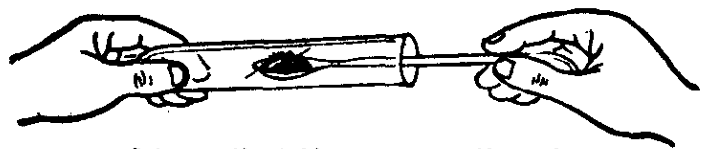
\includegraphics[width=0.6\textwidth]{../pic/czhx1-xssy-01}
    \caption{往试管里送入固体粉末}\label{fig:xssy-1}
\end{figure}

把块状的药品或密度较大的金属颗粒放入玻璃容器时,应该先把容器横放,
把药品或金属颗粒放入容器口以后,再把容器慢慢地竖立起来,
使药品或金属颗粒缓缓地滑到容器的底部,以免打破容器。

\textbf{学生练习}

(1) 用药匙的一端把固体粉末放入一个干燥的试管里(固体粉末可用实验室回收的药品或沙子等物代替)。
再练习把较重的颗粒放入另一个试管里。

(2) 把固体粉末放在折叠成槽状的纸条上,然后送入试管底部(图 \ref{fig:xssy-2} )。


\begin{figure}[htbp]
    \centering
    \begin{minipage}[b]{7cm}
        \centering
        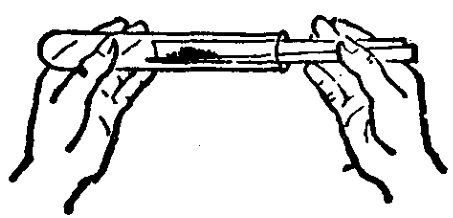
\includegraphics[width=6cm]{../pic/czhx1-xssy-02}
        \caption{用纸槽往试管里送入固体粉末}\label{fig:xssy-2}
    \end{minipage}
    \qquad
    \begin{minipage}[b]{7cm}
        \centering
        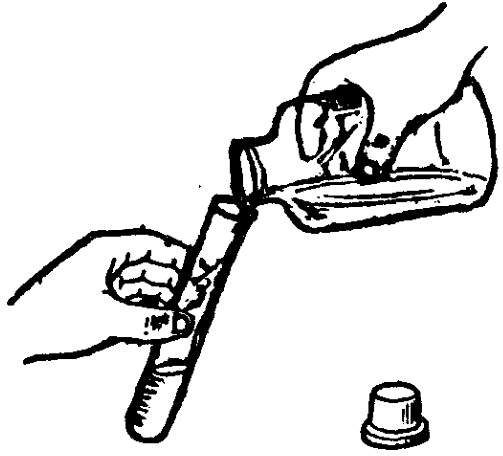
\includegraphics[width=6cm]{../pic/czhx1-xssy-03}
        \caption{液体的倾倒}\label{fig:xssy-3}
    \end{minipage}
\end{figure}


4. 液体药品的取用

液体药品通常盛在细口瓶里。取用的时候,先把瓶塞拿下,倒放在桌上。
然后一手拿起瓶子(瓶上的标签应向着手心,以免倒完药品后,残留在瓶口的药液流下来,腐蚀标签),
另一手略斜地持试管,使瓶口紧挨着试管口(图 \ref{fig:xssy-3} ),把液体缓缓地倒入试管里。

需用液体倒完后,立即盖紧瓶塞,把瓶子放回原处,要注意使瓶上的标签向外。

\textbf{学生练习}

(1) 取一个试管和一个盛有水的细口瓶,按图3 所示练习倾倒液体。

(2) 往三个试管里依次倒入下列容积的水: 1/3 试管, 1/4 试管, 1/5 试管。
要求对每种容积反复练习多次,直到比较熟练为止。


5. 浓酸、浓碱的使用

使用浓酸、浓碱等腐蚀性的药品,必须\zhongdian{特别小心},防止沾到皮肤上或洒在衣服上。

如果酸流到桌上,可以立即往酸里加适量的碳酸氢钠溶液,直到不发生气泡为止。
如果碱溶液流到桌上,可以立即往碱里加适量的稀醋酸来中和。
然后,先用水冲洗桌子,再用抹布擦干净。
如果只有少量酸或碱溶液滴到桌上,可以立即用湿抹布擦净,再用水冲洗抹布。

如果酸沾到皮肤上,立即用较多的水冲洗(皮肤上不慎洒上浓硫酸,不得先用水冲洗,
而要根据情况迅速用布拭去,再用水冲洗), 再涂上 3—5\% 的碳酸氢钠溶液。
如果碱溶液沾到皮肤上,也要用较多的水冲洗,再涂上硼酸溶液。

要注意保护眼睛。万一眼睛里溅进了酸或碱溶液,要立刻用水冲洗(切不可用手揉眼)。
洗的时候要眨眼睛,同时要报告教师,必要时找医生治疗。


\subsection{物质的称量和液体的量取}

1. 托盘天平的使用

托盘天平由托盘(分左右两个)、指针、标尺、调节零点的螺丝、游码、刻度尺等组成(图 \ref{fig:xssy-4})。
托盘天平只能用于粗略的称量,能称准到 $0.1$ 克。

\begin{figure}[htbp]
    \centering
    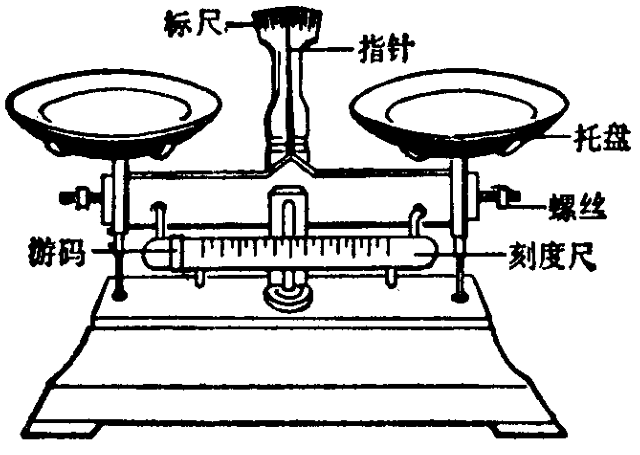
\includegraphics[width=0.5\textwidth]{../pic/czhx1-xssy-04}
    \caption{托盘天平}\label{fig:xssy-4}
\end{figure}

(1) 称量前先把游码放在刻度尺的零处,检查天平的摆动是否到达平衡。
如果已到达平衡,指针摆动时先后指示的标尺上的左、右两边的格数接近相等,指针静止时则应指在标尺的中间。
如果天平的摆动未到达平衡,可以调节左、右的螺丝,使摆动到达平衡。
想一想,如果指针偏向左边,哪一边的托盘的质量较大?应怎样调节螺丝?为什么?

(2) 称量物不能直接放在托盘上。可在两个托盘上各放一张大小相同的同种的纸,然后把要称量的药品放在纸上称量。
潮湿的或具有腐蚀性的药品必须放在玻璃器皿(如表面皿、烧杯)里称量。

(3) 把称量物放在左盘,砝码放在右盘。砝码要用镊子夹取。
先加质量大的砝码,再加质量小的砝码,最后可移动游码,直到天平摆动到达平衡为止。
记录所加砝码和游码的质量。

(4) 称量完毕后,应把砝码放回砝码盒中,把游码移回零处。

\textbf{学生练习}

(1) 把托盘天平放在平坦的桌面上,调节零点。
在天平两边的托盘上各放一张大小相同的同种的纸,观察零点有无变化?
想一想,右托盘上放纸的目的是什么?

(2) 称量 1 药匙食盐(或用沙子等物代替)的质量。记录数据。

(3) 计算 3 药匙食盐的质量。把该质量的砝码放好后再加食盐。
应练习逐渐加食盐到天平摆动到达平衡。
当食盐的量只缺很少时,可用左手拿药匙,右手拍左手手腕,
靠药匙振动而掉下的少量食盐来加足药量。

2. 量筒的使用

取用一定量的液体药品,可用量筒量出体积。量液体时,量筒必须放平稳,
而且使视线与量筒内液体的凹液面的最低处保持水平(图 \ref{fig:xssy-5}),
再读出所取液体的体积数。

\begin{figure}[htbp]
    \centering
    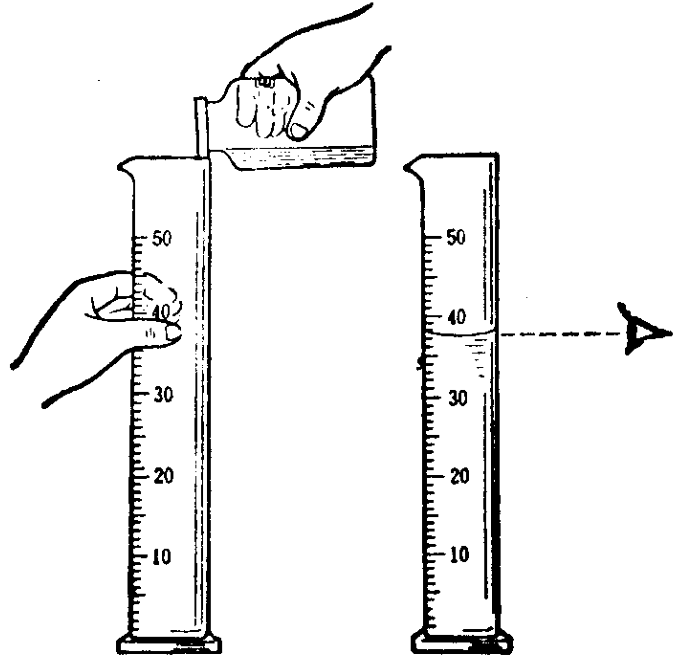
\includegraphics[width=0.5\textwidth]{../pic/czhx1-xssy-05}
    \caption{液体的量取}\label{fig:xssy-5}
\end{figure}


\textbf{学生练习}

(1) 取一个 10 毫升的量筒,把水加到指定容积的刻度( 10 毫升、5 毫升)。反复练习。
当水的量接近所需容积刻度线时,可用一干净滴管取少量水滴入量筒(不要把滴管伸入量筒内或接触筒壁)。

(2) 用 10 毫升的量筒量取 2 毫升的水。把水倒入一个试管里,记住液面在试管里的高度,
然后把试管里的水再倒回 10 毫升的量筒里。用试管再先后 3 次移取约 2 毫升的水到量筒中。
最后读一下量筒中水的体积数。

(3) 用滴管取少量水,向量筒里逐滴加水至 1 毫升,数一数需要多少滴?
再向试管里滴入约 1 毫升水,记住液面在试管里的高度。


\subsection{物质的加热}

1. 使用酒精灯的方法

(1) 使用酒精灯以前,要检查一下灯芯,如果灯芯顶端不平或已烧焦,就要剪去少许;
还要检查灯里有无酒精。向灯里添加酒精,不可超过酒精灯容积的 2/3 。
\zhongdian{绝对禁止向燃着的酒精灯里添加酒精},以免失火。

(2) 为了得到适当大小的火焰,先要调整灯芯,然后用火柴点燃(图 \ref{fig:xssy-6}, I)。
\zhongdian{绝对禁止拿酒精灯到另一已经燃着的酒精灯上去点火}(图 \ref{fig:xssy-6} ,II), \zhongdian{以免失火}。

\begin{figure}[htbp]
    \centering
    \begin{minipage}[b]{4cm}
        \centering
        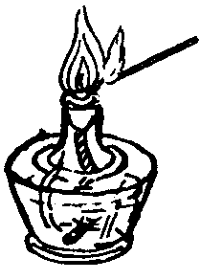
\includegraphics[width=3cm]{../pic/czhx1-xssy-06-1}
        \caption*{I}
    \end{minipage}
    \qquad
    \begin{minipage}[b]{4cm}
        \centering
        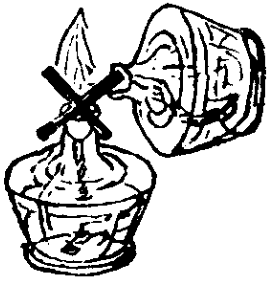
\includegraphics[width=3.5cm]{../pic/czhx1-xssy-06-2}
        \caption*{II}
    \end{minipage}
    \qquad
    \begin{minipage}[b]{4cm}
        \centering
        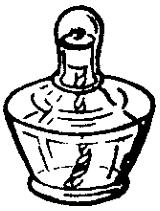
\includegraphics[width=3cm]{../pic/czhx1-xssy-06-3}
        \caption*{III}
    \end{minipage}
    \caption{酒精灯的使用}\label{fig:xssy-6}
\end{figure}

(3) 酒精灯的火焰必须用灯帽盖灭(图 \ref{fig:xssy-6}, III), \zhongdian{不可用嘴吹灭}。
如果用嘴吹,可能引起灯内酒精的燃烧,发生危险。

酒精灯不用的时候,必须盖上灯帽。不然洒精会蒸发掉,这样不但浪费酒精,
而且灯芯上留有水分(商品酒精都含有少量水),以后就不易点燃或燃烧不好。

使用酒精灯要随时小心,不要碰倒。
万一洒出的酒精在桌上燃烧起来,应该立刻用湿抹布扑盖或撒沙土扑灭。

2. 给物质加热

\begin{wrapfigure}[10]{r}{5cm}
    \centering
    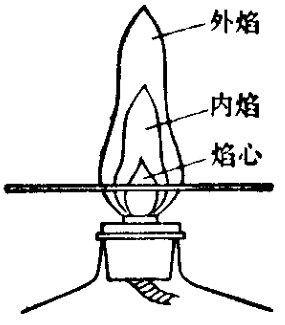
\includegraphics[width=4cm]{../pic/czhx1-xssy-07}
    \caption{酒情灯的灯焰}\label{fig:xssy-7}
\end{wrapfigure}

(1) 酒精灯的火焰可分焰心、内焰、外焰三个部分。
如将一根火柴梗迅速放进酒精灯的火焰中,象图 \ref{fig:xssy-7} 那样平放着。等 1—2 秒钟拿出来,
可以看到处在火焰外层(外焰)的部分最先碳化。
因为外焰燃烧充分,所以外焰温度最高,内焰燃烧不充分,温度较低,焰心温度最低。
加热时,应把受热物质放在外焰部分。


(2) 给液体加热可以用试管、烧瓶、烧杯、蒸发皿;给固体加热可以用干燥的试管、坩埚、烧瓶等。

(3) 给试管里的物质加热,必须使用试管夹。
将试管夹从试管底部往上套,夹在试管的中上部。
用手拿住试管夹的长柄,不要把拇指按在短柄上。
给烧瓶或烧杯里的物质加热,要放在铁架台的铁圈上(烧瓶要用夹子夹住颈部), 垫上石棉网,
使烧瓶或烧杯受热均匀,不致破裂。
用坩埚加热,要把它放在泥三角上。如需移动坩埚,必须用坩埚钳夹住。
用蒸发皿加热,可把它放在铁架台上大小适宜的铁圈上。加热后不要直接用手拿,可使用坩埚钳夹取。

(4) 如果被加热的玻璃容器外壁有水,应在加热前擦拭干净,然后加热,以免容器炸裂。

(5) 加热的时候,不要使玻璃容器的底部跟灯芯接触,以免容器破裂(图 \ref{fig:xssy-8})。
烧得很热的玻璃容器,不要立即用冷水冲洗或放在桌上,否则可能破裂。

\begin{figure}[htbp]
    \centering
    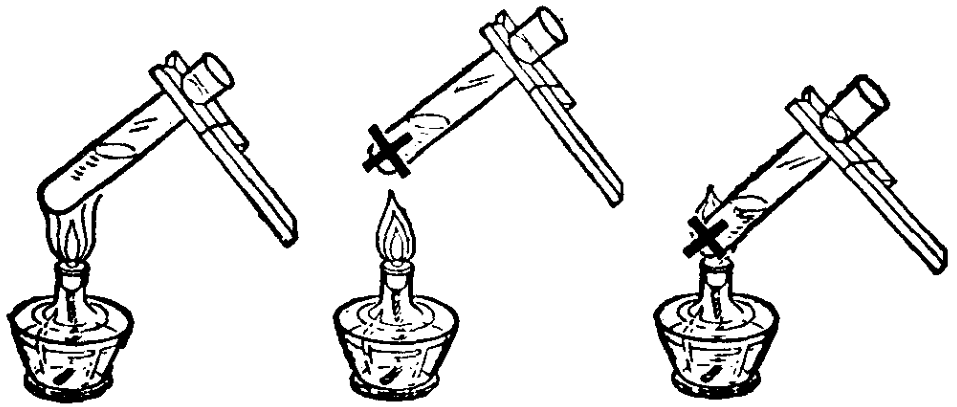
\includegraphics[width=0.7\textwidth]{../pic/czhx1-xssy-08}
    \caption{用酒精灯给物质加热}\label{fig:xssy-8}
\end{figure}


(6) 给试管里的固体加热,应该使试管在火焰上移动(如果试管需要固定,可移动酒精灯),
试管均匀受热后,再将火焰固定在放固体的部分加热。

(7) 给试管里的液体加热,液体体积一般不要超过试管容积的 1/3,
加热时,试管要倾斜(跟桌面成 $45^\circ$ 角)。
先使试管均匀受热,然后小心地在试管里液体的中下部加热,并且不时地上下移动试管。
\zhongdian{为避免试管里液体沸腾喷出伤人,加热时切不可使试管口对着自己或旁人}。

\textbf{学生练习}

(1) 检查一个酒精灯的灯芯和里面的酒精液面是否符合要求。
如不符合要求,请进行调整。
用火柴点燃酒精灯,观察它的火焰,然后熄灭。

(2) 取一个试管,加入 3 毫升的水,用试管夹夹住,按上述要求进行加热。
注意不要使试管口对着自己或别人。
观察在试管底部的某一部分集中加热和不时地上下移动试管加热时,液体沸腾的现象有什么不同。
想一想,为什么要 “不时地上下移动试管”?


\subsection{液体的过滤}

1. 过滤器的准备

取一张圆形滤纸(图 \ref{fig:xssy-9},I), 先折成半圆(图 \ref{fig:xssy-9}, II),再折成四等分(图\ref{fig:xssy-9}, III),
然后打开成圆锥形,把圆锥形的滤纸尖端向下,放入漏斗里,滤纸的边缘应比漏斗口稍低
(大约低 5 毫米,多余的滤纸应该剪去)。然后用手压住,用水润湿,
使滤纸紧贴着漏斗的内壁,中间不要留有气泡(图 \ref{fig:xssy-9}, IV)。
这样就做成一个过滤器。

\begin{figure}[htbp]
    \centering
    \begin{minipage}[b]{3cm}
        \centering
        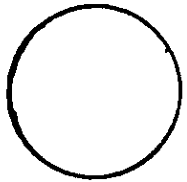
\includegraphics[width=2cm]{../pic/czhx1-xssy-09-1}
        \caption*{I}
    \end{minipage}
    \qquad
    \begin{minipage}[b]{3cm}
        \centering
        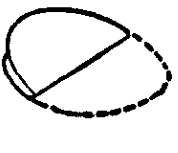
\includegraphics[width=2cm]{../pic/czhx1-xssy-09-2}
        \caption*{II}
    \end{minipage}
    \qquad
    \begin{minipage}[b]{3cm}
        \centering
        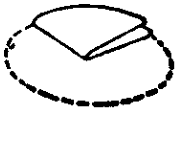
\includegraphics[width=2cm]{../pic/czhx1-xssy-09-3}
        \caption*{III}
    \end{minipage}
    \begin{minipage}[b]{3cm}
        \centering
        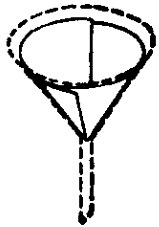
\includegraphics[width=2cm]{../pic/czhx1-xssy-09-4}
        \caption*{IV}
    \end{minipage}
    \caption{过滤器的准备}\label{fig:xssy-9}
\end{figure}


2. 过滤的方法

\begin{wrapfigure}[13]{r}{5cm}
    \centering
    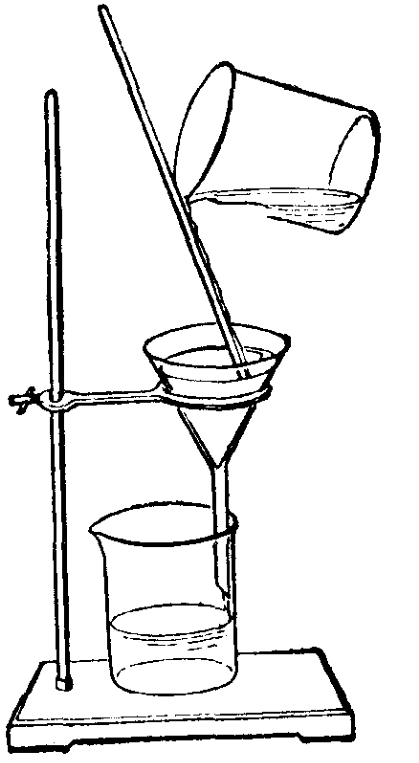
\includegraphics[width=4cm]{../pic/czhx1-xssy-10}
    \caption{过滤的方法}\label{fig:xssy-10}
\end{wrapfigure}

(1) 把过滤器放在铁架台的铁圈(或漏斗架)上,调整高度,
使漏斗下端的管口靠紧烧杯的内壁(图 \ref{fig:xssy-10})。
这样可以使滤液沿烧杯内壁流下,不致溅出来。


(2) 按照图 \ref{fig:xssy-10} 所示,使液体沿着玻璃棒流进过滤器(玻璃棒的末端要轻轻地斜靠在有三层滤纸的一边)。
漏斗里的液体的液面要低于滤纸的边缘,如果液体的液面高于滤纸的边缘,
液体就会从滤纸和漏斗壁之间流下,使固体混入滤液。

(3) 如果滤液仍然浑浊,应该把滤液再过滤一次。

3. 洗涤沉淀的方法

洗涤滤纸上的沉淀,可以照图 \ref{fig:xssy-10} 所示,向漏斗里注入少量水,使水面浸过沉淀物,等水滤出以后,
再次加水洗涤,连洗几次,即可把沉淀洗干净。

\textbf{学生练习}(也可以结合实验一进行)

做一个过滤器。过滤一杯混有泥沙的水。



\subsection{仪器的装配\footnotemark}
\footnotetext{化学实验基本操作五、六的学生练习可结合后面的学生实验进行。}

装配仪器首先要看清楚装置图, 然后选择仪器和零件,一件一件地连接起来,
最后要检查装配好的装置是不是严密不漏气(即检查气密性)。

1. 仪器和零件的连接

(1) 把玻璃管插入带孔像皮塞或软木塞的方法 \quad
左手拿橡皮塞或软木塞,右手拿玻璃管(靠近要插入塞子的一端),
先把玻璃管要插入塞子的一端用水润湿(图 \ref{fig:xssy-11}),
然后稍稍用力转动(小心!不要使玻璃管折断,以致刺破手掌),使它插入。


\begin{figure}[htbp]
    \centering
    \begin{minipage}[b]{7cm}
        \centering
        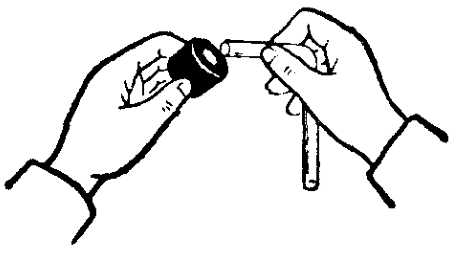
\includegraphics[width=5cm]{../pic/czhx1-xssy-11}
        \caption{把坡璃管插入橡皮塞的孔里}\label{fig:xssy-11}
    \end{minipage}
    \qquad
    \begin{minipage}[b]{7cm}
        \centering
        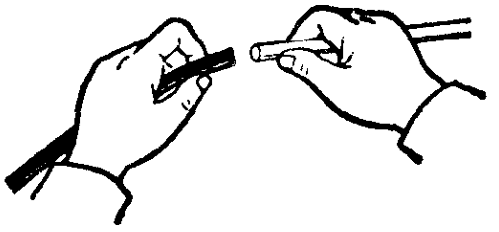
\includegraphics[width=5cm]{../pic/czhx1-xssy-12}
        \caption{在玻璃管上套上橡皮管}\label{fig:xssy-12}
    \end{minipage}
\end{figure}

(2) 使玻璃管跟橡皮管连接的方法 \quad 左手拿橡皮管,
右手拿玻璃管(图 \ref{fig:xssy-12}), 先把玻璃管口用水润湿,稍稍用力把玻璃管插入橡皮管。

\begin{wrapfigure}[8]{r}{6cm}
    \centering
    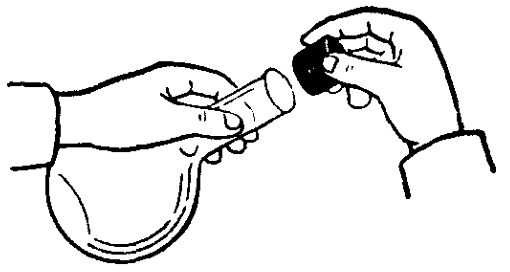
\includegraphics[width=5cm]{../pic/czhx1-xssy-13}
    \caption{用橡皮塞塞住烧瓶}\label{fig:xssy-13}
\end{wrapfigure}

(3) 在烧瓶口塞橡皮塞的方法 \quad 左手拿烧瓶颈,右手拿橡皮塞慢慢转动,塞进瓶口(图 \ref{fig:xssy-13})。
切不可把烧瓶放在桌上再使劲塞进塞子。因为这样做容易压破烧瓶。
在试管口塞橡皮塞,也要用同样的方法。


2. 装置的气密性的检查

要检查图 \ref{fig:xssy-14} 的装置是不是漏气,可以把导管的一端浸入水里,用手掌紧贴烧瓶的外壁。
如果装置不漏气,烧瓶里的空气受热膨胀,导管口就有气泡冒出(图 \ref{fig:xssy-14},I)。
把手移开,过一会儿烧瓶冷却,水就升到导管里,形成一段水柱(图 \ref{fig:xssy-14},II)。

\begin{figure}[htbp]
    \centering
    \begin{minipage}[b]{7cm}
        \centering
        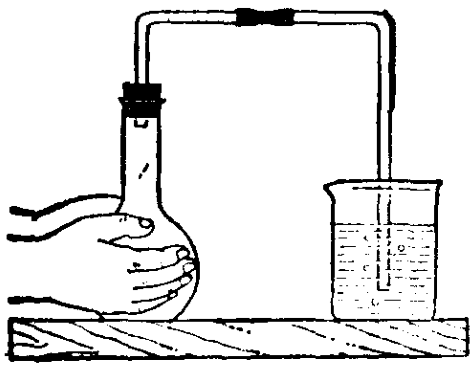
\includegraphics[width=5cm]{../pic/czhx1-xssy-14-1}
        \caption*{I}
    \end{minipage}
    \qquad
    \begin{minipage}[b]{7cm}
        \centering
        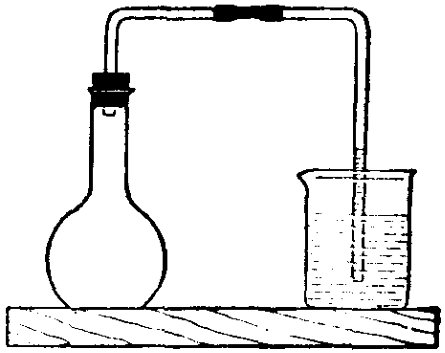
\includegraphics[width=5cm]{../pic/czhx1-xssy-14-2}
        \caption*{II}
    \end{minipage}
    \caption{检验装置的气密性}\label{fig:xssy-14}
\end{figure}

如果发现装置漏气,必须找出漏气的原因,并进行调整、修理,或更换零件。



\subsection{玻璃仪器的洗涤}

做实验必须用干净的玻璃仪器,否则会影响实验的效果。

做完实验,应该立刻把用过的玻璃仪器洗刷干净。

洗涤试管或烧瓶,可以注入半管或半瓶水,稍稍用力振荡,把水倒掉(图 \ref{fig:xssy-15}),照这样连洗数次。
如果内壁附有不易洗掉的物质,可以用试管刷刷洗。
刷洗时,使试管刷在盛水的试管里转动或上下移动,但用力不能过猛,否则容易把试管底弄破。


\begin{figure}[htbp]
    \centering
    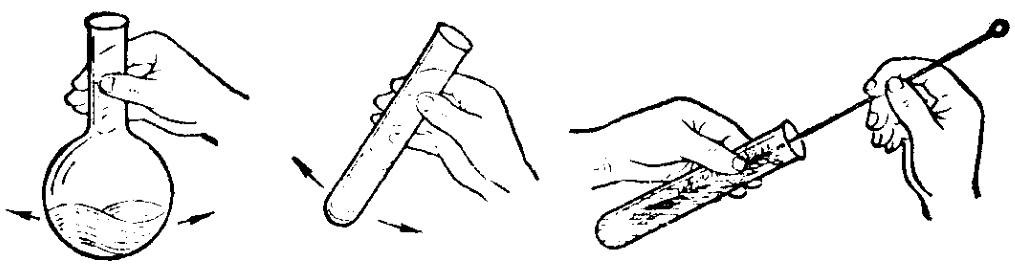
\includegraphics[width=0.7\textwidth]{../pic/czhx1-xssy-15}
    \caption{玻璃仪器的洗涤}\label{fig:xssy-15}
\end{figure}

玻璃仪器里如附有不溶于水的碱、碳酸盐、碱性氧化物等物质,可以先加稀盐酸溶解,再用水冲洗。
玻璃仪器里如附有油脂,可以先用热的纯碱(碳酸钠)溶液洗,再用试管刷刷洗,
也可用试管刷蘸少量去污粉或洗衣粉刷洗,然后用水把试管冲洗干净。

玻璃仪器洗过以后,如果内壁上附着的水均匀了,既不聚成水滴,也不成股流下,这才算洗干净了。

洗干净的玻璃仪器,应该倒放在平稳的地方,或放在试管架上晾干。

实验完毕,导管、橡皮塞等其它零件,也要用水洗干净。

